% ============================================================================
% PAQ living paper — comprehensive, honest, ongoing-research document.
% NOT a camera-ready submission: page limits do not bind; completeness and
% honesty do. Compiled with tectonic (see README_BUILD.md); any full TeX Live
% pdflatex+bibtex also works.
% Sources of every number: research/paq_verdict.json, research/paq_t_gate_verdict.json,
% research/paq_results.jsonl, the design notes under research/design_notes/, and
% research/MM_LANES/CROSS_LANE_LOG.md in the BASED repo. Figures are generated by
% scripts/paq_figs.py from those JSONs (nothing hand-entered).
% ============================================================================
\documentclass[11pt,letterpaper]{article}
\usepackage[margin=1in]{geometry}
\usepackage{amsmath,amssymb}
\usepackage{graphicx}
\usepackage{booktabs}
\usepackage{multirow}
\usepackage{tabularx}
\usepackage{xcolor}
\usepackage{algorithm}
\usepackage{algpseudocode}
\usepackage{caption}
\usepackage{natbib}
\usepackage{microtype}
\usepackage[colorlinks=true,linkcolor=blue!60!black,citecolor=blue!60!black,urlcolor=blue!60!black]{hyperref}

\graphicspath{{figures/}}
\captionsetup{font=small,labelfont=bf}

\newcommand{\paq}{\textsc{PAQ}}
\newcommand{\paqt}{\textsc{PAQ-T}}
\newcommand{\lb}{\mathrm{LB}_{95}}
\newcommand{\statusbox}[2]{\noindent\fbox{\parbox{0.97\linewidth}{\textbf{#1}\quad #2}}\medskip}

\title{\textbf{PAQ: Prefill-Once, Ask-Many}\\[2mm]
\large Reversible, query-conditioned page selection for multi-query document VQA\\[1mm]
\normalsize A living research document --- current state, honest negatives, and roadmap\\[1mm]
\small (status: 2026-07-15; this document tracks ongoing work and is updated as results land)}
\author{BASED-MM program}
\date{July 15, 2026}

\begin{document}
\maketitle

% ----------------------------------------------------------------------------
\begin{abstract}
\noindent
Real document-VQA benchmarks are \emph{multi-query}: one long document is prefilled once and
asked many different questions (in our pinned evaluation sets, 5.5--5.8 gold-bearing questions per
document). Standard KV-cache eviction commits to \emph{one} compressed context and reuses it for
every question. We study \paq{} (``Prefill-once, Ask-many''): retain the coarse document prefill
and, \emph{per query}, re-select a small page subset with the reader's own question$\to$page
attention, then reread those pages at full resolution. The axis we test is \textbf{reversibility}
--- per-query re-selection versus commit-once selection --- not query-awareness.

\textbf{What is confirmed.} On a 903-query confirmatory run (80 documents per cell, both cells,
document-clustered inference), per-query re-selection beats \emph{the identical scorer committed
once} (pooled accuracy $+0.210$, 95\% CI $[+0.168, +0.250]$) and a strong gold-informed static
subset ($+0.106$, $[+0.067, +0.141]$) --- on both cells, surviving an independent-extension check
on the 50 new documents per cell and a worst-case treatment of 4 timeout-missing queries.
The same fresh-over-stale pattern also holds for the retrieval scorer tested here (ColQwen2 fresh
$0.423$ vs.\ stale $0.178$ pooled).

\textbf{What is equally true and reported with the same prominence.} As a page selector, \paq{}
\emph{loses} head-to-head to a strong trained visual retriever: ColQwen2 re-ranked per query beats
\paq{} by $\approx$10 accuracy points at matched page budget (pooled $-0.099$, 95\% CI
$[-0.129, -0.072]$), on every reported stratum. Moreover, CAPS (ACL~2026) has already published
attention-based page selection beating ColPali-family retrieval on these same benchmarks --- the
page-level \emph{method} is scooped. A zero-shot expert-head variant (\paqt{}) reaches
\emph{recall} parity with ColQwen2 ($0.674$/$0.628$ vs.\ $0.664$/$0.536$ per cell), but its
accuracy read-out is still pending, its head is selected using gold recall on complementary
document folds, and expert-head selection is CAPS's technique.

\textbf{What this document is.} An honest consolidation of an ongoing project: the confirmed
multi-query reversibility result, the first \emph{executed} retrieval-vs-selection panel on
MMLongBench-Doc/LongDocURL at 64K context, the evidence that selection quality limits \paq{} v1,
and the resulting \emph{hypothesis} that selection below whole-page granularity is the next useful
direction. The region- and token-level extensions have planning odds of 15--35\%, depending on the
extension. They are proposals, not results.
\end{abstract}

\tableofcontents
\newpage

% ============================================================================
\section{Introduction}\label{sec:intro}

\subsection{The problem}
Long-context vision--language models (VLMs) can read an entire multi-page document, but they pay
for every page on every question. The standard efficiency response, inherited from single-query
text benchmarks, is to \emph{evict}: keep a compact subset of the KV cache (SnapKV, H2O, FastV,
LOOK-M, KVzip) and decode against it \citep{li2024snapkv,zhang2023h2o,chen2024fastv,wan2024lookm,kim2025kvzip}.
Eviction is a \emph{single, irreversible commitment}: whatever subset is kept must serve every
future question about that document.

\subsection{The multi-query regime}
Document assistants are not asked one question. The two long-document VQA benchmarks we use are
natively multi-query: grouping the 64K splits by source document, MMLongBench-Doc
\citep{ma2024mmlongbench} averages $\approx 6.97$ questions per document and LongDocURL
\citep{deng2025longdocurl} $\approx 3.6$; inside our pinned evaluation subsets (which require
$\geq 3$ gold-bearing questions per document) the averages are 5.50 and 5.79 respectively
(Table~\ref{tab:pins}). Different questions need different pages, so a subset committed for
question~1 is \emph{stale} for question~5.

\subsection{The question this project asks}
\begin{quote}
\emph{At a matched page budget on long multimodal documents, does per-query
\textbf{re-selection} of context beat a \textbf{commit-once} selection --- and can a
training-free, reader-internal selector compete with a dedicated trained retriever?}
\end{quote}
The answer, on the evidence in this document, is split, and we state it up front:
\begin{itemize}
  \item \textbf{Yes} to reversibility: re-selection beats commit-once, robustly, on both cells,
        for our scorer \emph{and} for a retrieval scorer (\S\ref{sec:results-isolation},
        \S\ref{sec:results-retrieval}). This is the confirmed contribution.
  \item \textbf{No} to the training-free selector: \paq{} loses to ColQwen2-fresh
        \citep{faysse2025colpali} by $\approx$10 accuracy points at page level
        (\S\ref{sec:results-retrieval}), and CAPS \citep{zhu2026caps} already published the
        page-level attention-selection method (\S\ref{sec:related-caps}). Zero-shot expert-head
        scoring closes the \emph{recall} gap (\S\ref{sec:results-paqt}) but accuracy parity is
        unverified.
  \item \textbf{Open} below page granularity: our current literature search leaves room for
        region- and token-level reversible selection. Whole-page routing can spend budget on
        non-evidence regions, but whether finer selection improves end-to-end accuracy is untested;
        the roadmap therefore remains explicitly speculative (\S\ref{sec:roadmap}).
\end{itemize}

\subsection{Reading guide}
\S\ref{sec:setup} fixes benchmarks and pins; \S\ref{sec:baselines} the executed baseline panel;
\S\ref{sec:method} the methods; \S\ref{sec:maths} the statistical machinery;
\S\ref{sec:algorithms} the algorithms; \S\ref{sec:results} all results (positive and negative,
with per-cell results primary and pooled results explicitly labelled); \S\ref{sec:related}
related work including the CAPS overlap; \S\ref{sec:roadmap} current state and roadmap;
\S\ref{sec:limitations} limitations. The
appendix carries the full panel, the adversarial review trail, and reproducibility pins.

% ============================================================================
\section{Benchmarks and setup}\label{sec:setup}

\subsection{Cells, documents, pins}
We evaluate on two cells: \textbf{LongDocURL} \citep{deng2025longdocurl} and
\textbf{MMLongBench-Doc} \citep{ma2024mmlongbench}, both consumed as page images (no OCR).
For each document we build the \emph{union of the benchmark's own-document pages} across that
document's queries (dropping cross-document 64K padding), so every query's evidence is present in
one prefill. Documents qualify if they have $\geq 3$ gold-bearing queries and $\leq 110$ union
pages ($\approx$64K tokens at read resolution); selection is seed-0 frozen.

Two pins exist: the 30-document/cell \emph{screen} pin and the 80-document/cell
\emph{confirmatory} pin. The screen pin is a strict prefix of the confirmatory pin (same seed,
same arrival order), which is why \S\ref{sec:results-isolation} additionally reports an
\emph{independent-extension} analysis on the 50 \emph{new} documents per cell --- the confirmatory
is not independent of the screen unless restricted to those. Both pins are sha-256--checksummed
and the harness verifies the screen pin byte-identically before use (Appendix~\ref{app:repro}).

\begin{table}[t]
\centering\small
\caption{The confirmatory evaluation pin (the numbers that should be cited). ``Complete queries''
are rows where every gated arm scored (complete-case pairing); 4 of 907 vision queries are missing
due to a per-document timeout (\S\ref{sec:results-missing}).}
\label{tab:pins}
\begin{tabular}{lcc}
\toprule
 & LongDocURL & MMLongBench-Doc \\
\midrule
Documents & 80 & 80 \\
Complete queries at gate ($b{=}5\%$) & 463 & 440 \\
Gold-bearing queries / document (pin) & 5.79 & 5.50 \\
Median (mean) union pages / document & 44 (45.0) & 28 (36.5) \\
Benchmark-level questions / document (64K split) & $\approx 3.6$ & $\approx 6.97$ \\
\bottomrule
\end{tabular}
\end{table}

\subsection{Reader, budgets, metric}
The reader is \textbf{Qwen3-VL-8B} \citep{qwen3vl2025}, frozen, eager attention. All selection
arms operate at a matched \emph{page} budget $b \in \{2.5\%, 5\%, 10\%\}$ of the document's pages
(the pre-registered gate budget is $b=5\%$); the selected pages are re-rendered at full resolution
and read. Accuracy is the benchmark's document-VQA scorer (exact/relaxed match by answer format).
Scope note: everything in this document is a \textbf{Qwen3-VL-8B case study}; no second VLM has
been run (\S\ref{sec:limitations}).

\subsection{The base-model ceiling}
A large fraction of queries receive no credit from this reader even when it is given
\emph{exactly} the annotated gold-evidence pages: on the confirmatory run the oracle-evidence arm
scores $0$ on
$317/903 = 35.1\%$ of queries and scores a full $1$ on only $407/903 = 45.1\%$ (the pre-specified
``answerable subset''). This limits absolute scores. Pairing controls for shared query difficulty,
but does not imply that the ceiling affects every selector equally; we report the answerable
subset only as a secondary view because it conditions on a model outcome. The oracle row is
\emph{not} a strict ceiling: \paq{} beats oracle-evidence on 28 queries, because a selected page
set can differ from the annotated gold set in ways that help the reader.

% ============================================================================
\section{Baselines: the executed panel}\label{sec:baselines}

Every arm below was actually run, per query, at matched page budget, on the same pinned data with
the same reader. The resulting panel directly compares retrieval and reader-internal selection on
MMLongBench-Doc/LongDocURL at 64K in the multi-query regime; our current literature search did not
identify an earlier executed panel with this exact scope. Table~\ref{tab:taxonomy} gives the
taxonomy; Appendix~\ref{app:panel} the full numbers.

\begin{table}[t]
\centering\small
\caption{Arm taxonomy. The load-bearing axis is \textbf{reversible} (re-select per query) vs.\
\textbf{commit-once} (one subset per document, reused for all its queries); the second axis is
deployability. Disclosed proxies are marked.}
\label{tab:taxonomy}
\begin{tabular}{llll}
\toprule
Arm & Reversible? & Deployable? & Role \\
\midrule
\paq{} (ours) & yes & yes & the method \\
attn\_max (ours, max-agg) & yes & yes & reported alternate aggregation \\
paq\_stale & no & yes & \textbf{isolation}: same scorer, committed once \\
gold\_frequency\_static & no & no (uses gold) & \textbf{isolation}: strong gold-informed static \\
ColQwen2-fresh & yes & yes & \textbf{strong deployable retrieval}, re-ranked per query \\
ColQwen2-stale & no & yes & retrieval committed once (same commit policy) \\
CLIP-fresh & yes & yes & cheaper retrieval control \citep{radford2021clip} \\
SnapKV-fresh & yes & yes & reference (weak port; beating it not required) \\
SnapKV-stale & no & yes & strongest stale family arm \\
H2O / FastV / LOOK-M / KVzip & no & yes & demoted query-blind controls (proxies, see text) \\
random / truncation & no & --- & controls \\
full-context / oracle-evidence & --- & --- & reference rows, \emph{not} competitors \\
\bottomrule
\end{tabular}
\end{table}

\paragraph{The demoted eviction family (disclosed proxies).} H2O uses accumulated received
attention; FastV is a \emph{context-only proxy} (canonical FastV is prompt-conditioned); LOOK-M
degenerates to H2O on image-only pages; KVzip is a \texttt{recv\_max} proxy for the reconstruction
pass of \citet{kim2025kvzip}. On these cells the whole family sits \emph{at or below random} page
recall, so beating it is not a claim we make --- they are query-blind controls, retained for
completeness, and a faithful-reconstruction KVzip would likely be stronger. The honest comparators
are \texttt{paq\_stale}, \texttt{gold\_frequency\_static}, SnapKV-stale/fresh, and the retrieval
arms.

\paragraph{On \texttt{gold\_frequency\_static}.} This arm keeps the top-$B$ pages by
\emph{gold-page frequency} across the document's queries. It uses gold labels, so it is not
deployable; it is a \emph{strong gold-informed static commitment} --- but it is \textbf{not}
provably accuracy-optimal and we do not call it ``best possible'' or a ``ceiling'' (an earlier
draft did; the claim was retracted under review, Appendix~\ref{app:reviews}).

\paragraph{Reference rows.} Full-context and oracle-evidence are reported for calibration only.
SnapKV-fresh (re-run per query) is a reference, not an upper bound; our port averages heads and
layers before pooling and is weaker than canonical SnapKV.

% ============================================================================
\section{Methods}\label{sec:method}

\subsection{\paq{}: coarse-to-fine page routing}\label{sec:method-paq}
\paq{} is training-free page routing over a frozen VLM:
\begin{enumerate}
  \item \textbf{Prefill once (per document).} Pages are rendered at coarse resolution
        ($\approx$3.5K visual tokens total, i.e.\ $\approx$70 tokens/page on a 50-page document)
        and prefilled once; the KV cache is retained. Attention statistics are captured by
        OOM-safe per-layer forward hooks (Algorithm~\ref{alg:hooks}).
  \item \textbf{Re-select per query.} The question is appended to the retained cache; the
        question rows' attention over page tokens (mean over heads, layers, and question tokens)
        is averaged over each page's token span to give a per-page score
        (Algorithm~\ref{alg:paq}). Keep the top pages at budget $b$.
  \item \textbf{Reread.} The selected pages are re-rendered at full resolution and the question
        is answered from them.
\end{enumerate}
\textbf{Scope, stated plainly:} this is \emph{page routing} --- coarse-score $\to$ pick pages
$\to$ full-resolution reread. It is \emph{not} token-level KV compression: we never decode from a
masked retained cache, and we claim no memory savings in v1. The estimand is query-conditioned
page selection at matched page budget.

\subsection{The reversibility framing and the isolation protocol}\label{sec:method-isolation}
``Query-aware selection beats query-agnostic eviction'' is both a known text result
\citep{tang2024quest} and a strawman risk (FastV and LOOK-M can attend to the question). We
therefore fix the axis to \textbf{reversibility}: every baseline runs its canonical scorer but is
deployed \emph{stale} --- committed once per document (query-aware members commit an aggregate
over the document's first $M=\min(3,k)$ queries) --- while \paq{} re-selects per query
(Algorithm~\ref{alg:stale}).

Reversibility is credited \emph{only} if \paq{} beats \textbf{both}
\begin{itemize}
  \item \texttt{paq\_stale}: \paq's \emph{own} scorer committed once. Identical scorer, identical
        budget; the only difference is reversibility, so the delta isolates the mechanism;
  \item \texttt{gold\_frequency\_static}: the strong gold-informed static, so the win is not an
        artifact of a weak committed selector.
\end{itemize}
This gate exists because a first, weaker gate (\paq{} vs.\ best-of-eviction-family) \emph{passed
and was then retracted}: adversarial review showed the family's stale arms were weak-static
artifacts (a gold-informed static nearly matched \paq{} in recall), so ``reversibility'' had not
been isolated. The two-comparator gate above was frozen before the confirmatory run
(Appendix~\ref{app:reviews} documents both review rounds).

\subsection{\paqt{}: expert-head, higher-resolution scoring (training-free CV)}\label{sec:method-paqt}
After the retrieval loss (\S\ref{sec:results-retrieval}) we tested how much of the gap is an
artifact of \paq's mean-aggregation and resolution starvation ($\approx$70 coarse tokens/page vs.\
ColQwen2's $\approx$1{,}024 patch embeddings/page). \paqt{} scores with (a) more scoring tokens
per page (256 tokens/page, 6{,}000-token target total --- a cap forced by encoder OOM on large
documents, not full page resolution), and (b) a single \emph{expert (layer, head)} chosen by
held-out-document cross-validation (Algorithm~\ref{alg:expert}) rather than the mean over all
heads. Expert-head selection is CAPS's technique \citep{zhu2026caps}; what is ours here is the
amortized multi-query architecture it plugs into. \paqt{} so far has a \emph{recall} result only
(\S\ref{sec:results-paqt}); the accuracy read-eval is pending. ``Training-free'' means no parameter
updates: choosing the head still uses gold recall on the complementary fold of the same benchmark,
so this is not unsupervised model selection.

% ============================================================================
\section{Definitions and statistical machinery}\label{sec:maths}

\paragraph{Matched page budget.} For a document with $n$ pages and budget fraction $b$, every arm
keeps
\begin{equation}
B \;=\; \max\!\bigl(1, \lfloor b \cdot n \rfloor\bigr)
\label{eq:budget}
\end{equation}
pages. Pages have unit budget weight in the executed vision harness, so this is the exact behavior
of its cumulative-budget selector; ties in score are broken by page index. The same selector code
path is used for every arm.

\paragraph{Gold-page recall at budget.} For query $q$ with nonempty annotated gold-page set $G_q$
and kept set $K_q$ ($|K_q| = B$),
\begin{equation}
\mathrm{recall}@b(q) \;=\; \frac{|K_q \cap G_q|}{|G_q|}.
\label{eq:recall}
\end{equation}
Reported recall is the query-macro mean of this fraction within a cell; it is not answer accuracy
and it is not the binary event ``at least one gold page retrieved.''

\paragraph{Commitment pressure.} For a document with $g$ distinct gold pages across its $k$
queries,
\begin{equation}
\mathrm{pressure} \;=\; \frac{g}{b \cdot n},
\label{eq:pressure}
\end{equation}
i.e.\ how many times over the $b$-budget capacity the document's queries collectively need.
This pre-registered quantity uses the fractional, pre-rounding capacity $bn$, whereas the executed
selector uses $B$ from Eq.~\eqref{eq:budget}. Thus pressure $>1$ means $g>bn$; when $bn\geq1$ this
also implies $g>B$ and no single $B$-page subset can contain every distinct annotated gold page.
For $bn<1$ and at rounding boundaries, pressure should be read as a continuous diagnostic rather
than a literal coverability test.
This was the pre-registered mechanism axis; the formal test of it \textbf{failed}
(\S\ref{sec:results-mechanism}) and it is retained as exploratory only.

\paragraph{Document-cluster paired bootstrap and $\lb$.} For arms $A$ and $C$, let
$d_q=s_A(q)-s_C(q)$ be their paired accuracy-score difference on query $q$. With two cells
$c\in\{1,2\}$ and $N_c$ queries in cell $c$, the pooled point estimate is
\begin{equation}
\widehat{\Delta}_{A-C}
= \frac{1}{2}\sum_{c=1}^{2}\left(\frac{1}{N_c}\sum_{q\in c} d_q\right).
\label{eq:pooled-delta}
\end{equation}
Queries of one document share the document \emph{and} the single stale subset, so bootstrapping
over queries would be anti-conservative pseudoreplication. All intervals therefore resample
\emph{documents} with replacement within each cell (10{,}000 draws, seed 0), recompute
Eq.~\eqref{eq:pooled-delta}, and take percentile endpoints. Per-cell intervals use the same
procedure with one cell. We define
\begin{equation}
\lb(\Delta) = \text{2.5th percentile of the bootstrap distribution of } \Delta,
\qquad
\mathrm{UB}_{95}(\Delta) = \text{97.5th percentile},
\label{eq:lb95}
\end{equation}
i.e.\ $\lb$ is the \textbf{lower end of a two-sided 95\% CI} (equivalently a one-sided 97.5\%
bound). An earlier label of ``one-sided 95\%'' was incorrect and has been fixed; the frozen gate
arithmetic never changed.

\paragraph{The isolation gate (pre-registered, frozen before the run).}
\begin{equation}
\textsc{Isolated} \iff
\lb\bigl(\widehat{\Delta}_{\text{\paq}-\texttt{paq\_stale}}\bigr) > 0
\;\;\wedge\;\;
\lb\bigl(\widehat{\Delta}_{\text{\paq}-\texttt{gold\_frequency\_static}}\bigr) > 0,
\label{eq:gate}
\end{equation}
using complete cases at $b = 5\%$. The frozen gate is pooled with equal cell weighting; the
per-cell intervals are corroborating analyses, not additional gate clauses. If either interval
includes zero, the evidence is insufficient to isolate a reversibility benefit; that outcome
would not establish equivalence between commit-once and per-query selection.

% ============================================================================
\section{Algorithms}\label{sec:algorithms}

\begin{algorithm}[t]
\caption{\paq{} per-query scorer and matched-budget selection (vision cells)}
\label{alg:paq}
\begin{algorithmic}[1]
\Require document pages $P_1,\ldots,P_n$; queries $q_1,\ldots,q_k$; budget $b$; frozen VLM (eager attention)
\State render all pages coarsely ($\approx\!3.5$K visual tokens total); prefill once; retain KV cache $C$
\State record image-token spans $s_1,\ldots,s_n$ for the pages
\For{each query $q_j$}
  \State forward only the tokenized question against $C$ (no re-prefill)
  \State via hooks: $\mathbf{a} \gets$ mean over layers, heads, and question rows of attention to
         each context position \Comment{Algorithm~\ref{alg:hooks}}
  \State per-page score $\mathrm{score}_j(p) \gets |s_p|^{-1}\sum_{t \in s_p} \mathbf{a}[t]$
         \Comment{\texttt{attn\_max} variant: max over $s_p$}
  \State $K_j \gets$ top-$B$ pages by $\mathrm{score}_j$, $B = \max(1,\lfloor b\,n\rfloor)$
         \Comment{Eq.~\eqref{eq:budget}; index tie-break}
  \State re-render pages $K_j$ at full resolution; answer $q_j$ from them
\EndFor
\end{algorithmic}
\end{algorithm}

\begin{algorithm}[t]
\caption{Commit-once (stale) vs.\ re-select (fresh) deployments --- the reversibility contrast}
\label{alg:stale}
\begin{algorithmic}[1]
\Require per-query score vectors $v_1..v_k \in \mathbb{R}^n$ from ANY scorer (\paq{}, SnapKV, ColQwen2)
\State \textbf{fresh (reversible):} for query $q_j$, select top-$B$ from $v_j$ \Comment{one subset per query}
\State \textbf{stale (commit-once):} $u \gets \frac{1}{M}\sum_{j\le M}\mathrm{minmax}(v_j)$ with
       $M=\min(3,k)$; select top-$B$ from $u$ once; reuse that subset for ALL $k$ queries
\State \textit{min-max normalization before averaging prevents any single query's magnitude from
       dominating the committed ranking; query order is frozen (arrival order).}
\State \textit{query-agnostic arms (H2O/FastV/LOOK-M/KVzip/random/trunc) are stale by construction
       (their score vector never sees a question).}
\end{algorithmic}
\end{algorithm}

\begin{algorithm}[t]
\caption{Expert-head selection with held-out-document CV (\paqt{}; gold-supervised selection on
the complementary fold, never on the scored documents)}
\label{alg:expert}
\begin{algorithmic}[1]
\Require per-(layer,head) question$\to$page scores; gold sets $G_q$; documents $D$ of one cell;
budget $b=5\%$
\State split $D$ into two folds by document (seed-0 shuffle)
\For{each fold $F$}
  \State $Q_{\mathrm{train}}\gets$ queries in $D\setminus F$
  \State on $Q_{\mathrm{train}}$: pick
         $(\ell^*,h^*)=\arg\max_{\ell,h}|Q_{\mathrm{train}}|^{-1}
         \sum_{q\in Q_{\mathrm{train}}}\mathrm{recall}@b_{\ell,h}(q)$
         \Comment{Eq.~\eqref{eq:recall}}
  \State evaluate $(\ell^*,h^*)$ on the held-out fold $F$
\EndFor
\State report query-macro held-out recall per cell
       \Comment{no weight updates; head choice does use training-fold gold labels}
\end{algorithmic}
\end{algorithm}

\begin{algorithm}[t]
\caption{OOM-safe per-layer-hook attention capture (the engineering that makes 64K scoring feasible)}
\label{alg:hooks}
\begin{algorithmic}[1]
\State register a forward hook on every language-decoder self-attention module (vision encoder excluded)
\State run the chunked prefill / question forward with \texttt{output\_attentions=False} under eager attention
\State inside each hook: catch the layer's $(1,H,q,k)$ attention tensor, reduce it immediately
       (fp32-accumulated column-sum for H2O, running max for KVzip, layer-2 last row for FastV,
       question-row mean for \paq), and \textbf{discard} it
\State peak memory $=$ ONE layer's attention. The naive all-layers
       \texttt{output\_attentions=True} path OOMs ($\approx$77\,GB at 128K text) or crashes vision cuDNN.
\State a capture guard hard-fails if no hook observed a 4D tensor (prevents silently scoring zeros)
\end{algorithmic}
\end{algorithm}

% ============================================================================
\section{Results}\label{sec:results}

The primary confirmatory numbers below come from \texttt{research/paq\_verdict.json} (903 complete
vision queries, 80 documents/cell, frozen v3 harness). The independent-extension, mechanism, and
fusion diagnostics come from the documented post-hoc scripts in Appendix~\ref{app:repro}; \paqt{}
numbers come from \texttt{research/paq\_t\_gate\_verdict.json}. Per-cell results are primary.
``Pooled'' inferential contrasts use the equal-cell statistic in Eq.~\eqref{eq:pooled-delta};
query-micro summaries are labelled separately.

% ----------------------------------------------------------------------------
\subsection{Confirmatory isolation: reversibility is real}\label{sec:results-isolation}

\statusbox{CONFIRMED}{Per-query re-selection beats the identical scorer committed once AND a
strong gold-informed static, on both cells, document-clustered, surviving independent-extension
and missingness worst-case checks.}

Table~\ref{tab:isolation} and Figure~\ref{fig:forest} give the gate result. At $b=5\%$:

\begin{table}[t]
\centering\small
\caption{Confirmatory isolation at $b{=}5\%$ on 903 complete queries (accuracy;
document-cluster paired bootstrap). Contrast rows report
$\Delta\,[\lb,\mathrm{UB}_{95}]$; the pooled column uses equal cell weighting.}
\label{tab:isolation}
\begin{tabular}{lccc}
\toprule
 & LongDocURL & MMLongBench-Doc & pooled (equal-cell) \\
\midrule
\paq{} accuracy & 0.385 & 0.258 & 0.322 \\
\texttt{paq\_stale} accuracy & 0.128 & 0.095 & 0.111 \\
\texttt{gold\_frequency\_static} accuracy & 0.278 & 0.154 & 0.216 \\
\midrule
\paq{} $-$ \texttt{paq\_stale} & $+0.257$ $[+0.184,+0.330]$ & $+0.163$ $[+0.126,+0.200]$ & $+0.210$ $[+0.168,+0.250]$ \\
\paq{} $-$ \texttt{gold\_freq\_static} & $+0.108$ $[+0.045,+0.164]$ & $+0.104$ $[+0.063,+0.144]$ & $+0.106$ $[+0.067,+0.141]$ \\
\midrule
Verdict & \multicolumn{3}{c}{\textsc{Reversibility isolated} (both $\lb > 0$, both cells and pooled)} \\
\bottomrule
\end{tabular}
\end{table}

At screen scale (30 documents/cell), the MMLongBench-Doc contrast against the static was
$-0.017$ with a CI including zero. It became positive at 80 documents; we treat that earlier
result as an underpowered screen, not as an independent replication.

\begin{figure}[t]
\centering
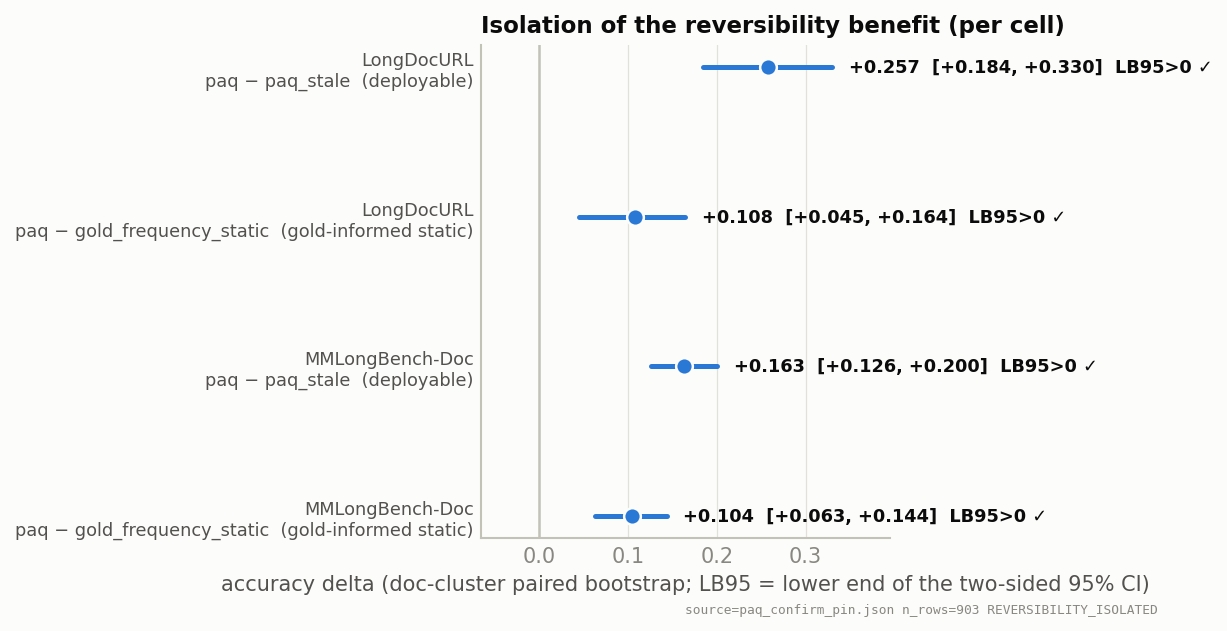
\includegraphics[width=0.9\linewidth]{fig_b_isolation_forest_light.png}
\caption{The statistical headline: per-cell forest of the two isolation contrasts at $b=5\%$.
Intervals are document-clustered two-sided 95\% CIs; all four exclude zero.}
\label{fig:forest}
\end{figure}

\paragraph{Independent extension (the screen is embedded in the confirmatory).} Because the
80-document pin contains the 30 screen documents, we re-ran the isolation statistics on the
\textbf{50 new documents per cell only} ($n=582$ queries): \paq{} $-$ \texttt{paq\_stale}
$+0.216$ $[+0.159,+0.269]$; \paq{} $-$ \texttt{gold\_frequency\_static} $+0.108$
$[+0.059,+0.150]$; per-cell static contrasts $+0.089$ $[+0.004,+0.162]$ (LongDocURL) and
$+0.127$ $[+0.083,+0.173]$ (MMLongBench-Doc). The result therefore also holds on the
out-of-screen extension.

\paragraph{Answerable subset (secondary).} On queries where oracle-evidence scores exactly 1
($n=407$, 137 docs): \paq{} 0.583 vs.\ \texttt{paq\_stale} 0.182 ($+0.395$ $[+0.324,+0.460]$)
and vs.\ the static 0.382 ($+0.204$ $[+0.135,+0.266]$). Reported secondarily because it
conditions on a model outcome.

\label{sec:results-missing}
\paragraph{Missingness.} 4 of 907 vision queries (MMLongBench-Doc document \texttt{mi\_phone},
queries 2--5) are missing due to a per-document timeout. Imputing them worst-case in either
direction leaves the gate verdict unchanged.

\paragraph{Budget curves.} Figure~\ref{fig:budget} shows accuracy at $b \in \{2.5, 5, 10\}\%$:
\paq{} dominates \texttt{paq\_stale} and the static at every budget on both cells, monotonically.
On LongDocURL, \paq{} at $b=10\%$ reaches 0.518 vs.\ full-context 0.546 --- reading 10\% of pages
recovers $\approx$95\% of full-context accuracy on that cell (not on MMLongBench-Doc: 0.317 vs.\
0.397).

\begin{figure}[t]
\centering
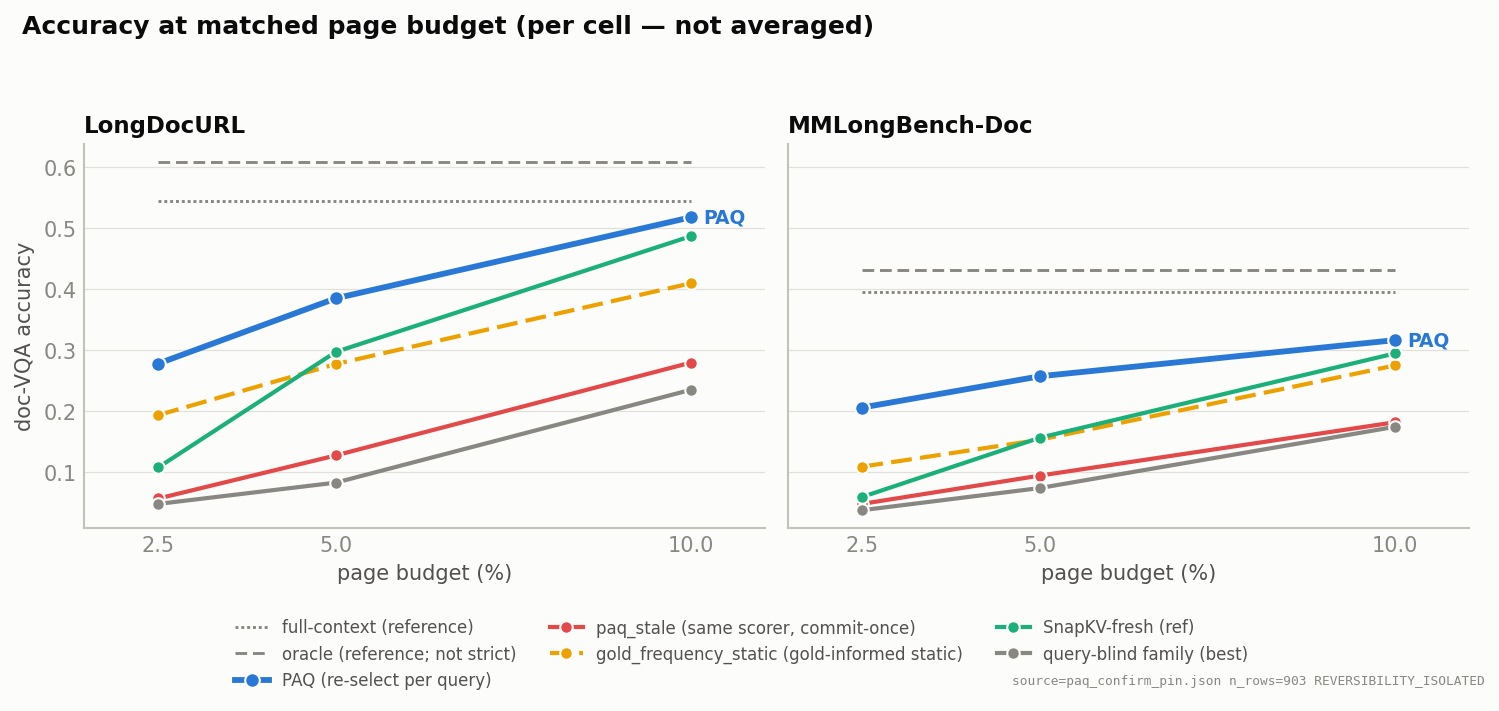
\includegraphics[width=\linewidth]{fig_a_budget_curves_light.png}
\caption{Accuracy at matched page budget, per cell (never averaged). Full-context and
oracle-evidence are recessive reference lines, not competitors; the ``query-blind family (best)''
line is the demoted control family's best member.}
\label{fig:budget}
\end{figure}

% ----------------------------------------------------------------------------
\subsection{The deployable retrieval comparison: \paq{} loses at page level}\label{sec:results-retrieval}

\statusbox{CONFIRMED NEGATIVE}{A strong trained visual retriever re-ranked per query beats \paq{}
by $\approx$10 accuracy points at matched page budget. This is the decisive result of the final
review round, reported with the same prominence as the positive.}

The adversarial AAAI-readiness review named one decisive missing experiment: a deployable
query-conditioned \emph{retrieval} baseline. We ran it: ColQwen2 \citep{faysse2025colpali}
(late-interaction MaxSim over page images; pages embedded once per document) fresh and stale, plus
CLIP \citep{radford2021clip} fresh, same reader, same budgets, all 903 queries. At $b=5\%$,
pooled, document-clustered (Table~\ref{tab:retrieval}, Figure~\ref{fig:retrieval}):

\begin{table}[t]
\centering\small
\caption{Deployable retrieval comparison at $b{=}5\%$ (accuracy; 903 complete queries).
\paq{} loses to ColQwen2-fresh on both cells. Fresh exceeds stale for both tested scorers.
The pooled arm means use equal cell weighting; contrast intervals are document-clustered.}
\label{tab:retrieval}
\begin{tabular}{lccc}
\toprule
 & LongDocURL & MMLongBench-Doc & pooled (equal-cell) \\
\midrule
ColQwen2-fresh & 0.512 & 0.328 & 0.420 \\
\paq{} & 0.385 & 0.258 & 0.322 \\
ColQwen2-stale (commit-once) & 0.216 & 0.138 & 0.177 \\
CLIP-fresh & 0.155 & 0.164 & 0.159 \\
full-context (reference) & 0.546 & 0.397 & --- \\
\midrule
\paq{} $-$ ColQwen2-fresh & \multicolumn{3}{c}{pooled $-0.099$ $[-0.129, -0.072]$ \; $\Rightarrow$ \; \textbf{\paq{} loses}} \\
\paq{} $-$ ColQwen2-stale & \multicolumn{3}{c}{pooled $+0.145$ $[+0.101, +0.185]$} \\
\paq{} $-$ CLIP-fresh & \multicolumn{3}{c}{pooled $+0.162$ $[+0.128, +0.197]$} \\
\bottomrule
\end{tabular}
\end{table}

\begin{figure}[t]
\centering
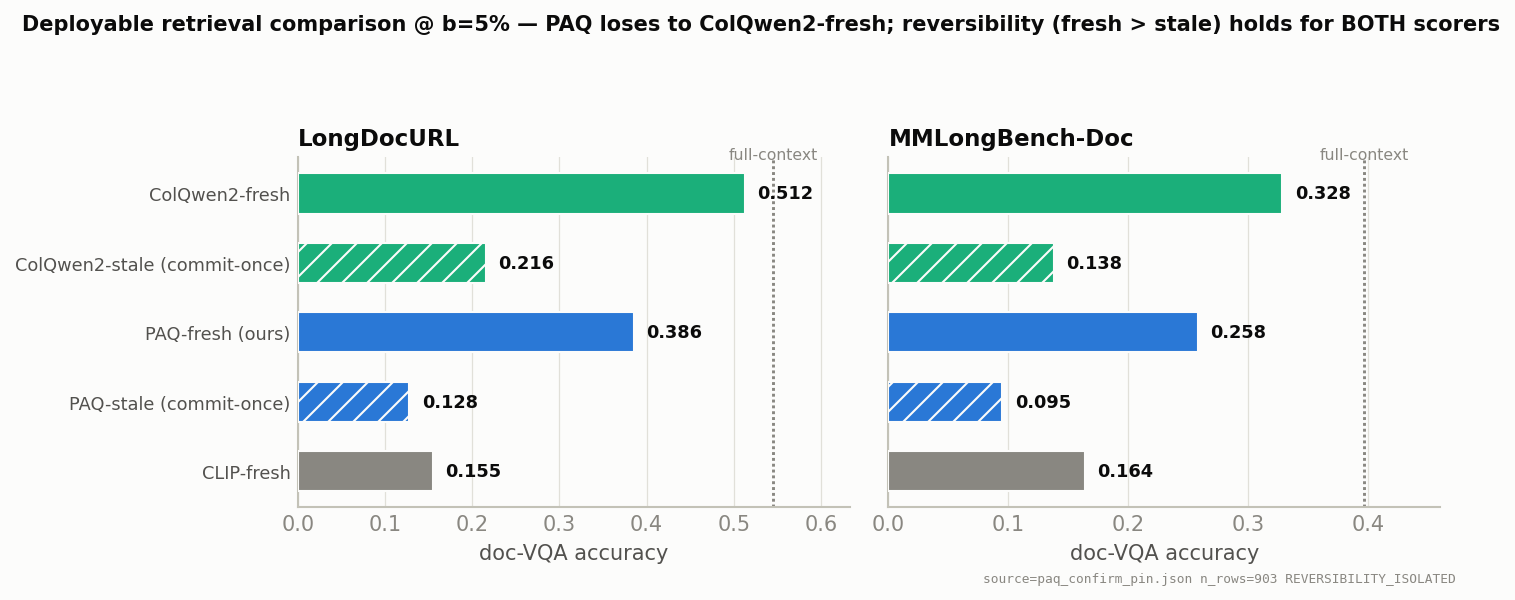
\includegraphics[width=\linewidth]{fig_e_retrieval_reversal_light.png}
\caption{The two honest facts in one picture, per cell: (i) ColQwen2-fresh beats \paq{}
(the $\approx$10pt loss); (ii) \emph{both} scorers collapse when committed once --- reversibility
is a general property of the multi-query regime, not a \paq{}-specific effect.}
\label{fig:retrieval}
\end{figure}

Three readings, all of which we stand behind:
\begin{enumerate}
  \item \textbf{\paq{} is not a superior page router.} The loss is $\approx$10 points, $\lb$
        well below zero, and it holds on every stratum we examined (single-gold $-0.110$,
        multi-gold $-0.086$; no question type where attention beats retrieval).
  \item \textbf{The reversibility pattern spans both tested scorer families.} On the
        query-micro summary, ColQwen2-fresh is 0.423 vs.\ 0.178 stale; the corresponding
        equal-cell means are 0.420 and 0.177. This reproduces the fresh-vs-stale collapse with a
        different scorer. It supports per-query reselection for attention- and retrieval-based
        systems in this evaluated regime; it is not a claim about every possible scorer.
  \item \textbf{The two existing outputs have limited complementarity.} A per-query oracle taking
        the better observed answer score from \{\paq{}, ColQwen2-fresh\} gains $+0.035$ pooled
        over ColQwen2-fresh ($\lb$ $+0.024$; $+0.041$/$+0.030$ per cell). Among the 419 queries
        where ColQwen2-fresh scores exactly zero, \paq{} scores one on only $\approx$6\%.
        This makes simple output routing low priority. It does \emph{not} upper-bound a fusion or
        reranker that selects a new page set, whose reader output could differ from both inputs.
\end{enumerate}

Gold-page recall is consistent with a coverage contribution to the loss: at $b=5\%$,
ColQwen2-fresh recalls 0.664/0.536 (per cell) vs.\ \paq{} 0.494/0.443. This observation motivated
the \paqt{} selection diagnostic (\S\ref{sec:results-paqt}); by itself it is not a causal
decomposition of the accuracy gap.

\paragraph{Why the loss redirects rather than ends the project.} Simply replacing mean
aggregation with a better page-level attention head is not a clean novelty route: CAPS has already
published expert-head attention selection on these benchmarks (\S\ref{sec:related-caps}). We
therefore treat \paqt{} as a diagnostic and defer the unexecuted below-page ideas to
\S\ref{sec:roadmap}, after the confirmed and negative evidence.

% ----------------------------------------------------------------------------
\subsection{Mechanism: demoted to exploratory}\label{sec:results-mechanism}

\statusbox{RETRACTED AS A CLAIM}{The pre-registered ``commitment-pressure gradient'' mechanism
FAILED its formal test; what replaced it is a corrected, two-part account of where the benefit
comes from.}

We had hypothesized the reversibility benefit concentrates in high-commitment-pressure documents
(Eq.~\eqref{eq:pressure}) and reverses under low pressure. The screen suggested this; the formal
document-clustered interaction test on the confirmatory does \textbf{not} support it: high$-$low
pressure difference $+0.042$ $[-0.048, +0.130]$ on \paq{}$-$static and $-0.015$
$[-0.116, +0.080]$ on \paq{}$-$\texttt{paq\_stale} --- both include zero. LongDocURL shows the
predicted direction without significance; MMLongBench-Doc's benefit is broad across pressure.
Figure~\ref{fig:pressure} is therefore labelled exploratory and this document makes no
mechanism-gradient claim.

An earlier ``reading quality, not coverage'' explanation was also \textbf{wrong}: \paq's
gold-recall exceeds the static's by $+0.092$ (the earlier ``recall $\approx$ static'' countercheck
was in error), and at \emph{matched} recall ($n=415$) \paq{} still beats the static by $+0.049$
$[+0.021, +0.076]$. The corrected descriptive statement is: \textbf{per-query re-selection has
higher gold coverage overall and higher downstream accuracy among queries with equal measured
gold recall}. The matched-recall analysis does not identify why the selected page sets differ or
establish a separate causal ``reading quality'' mechanism.

\begin{figure}[t]
\centering
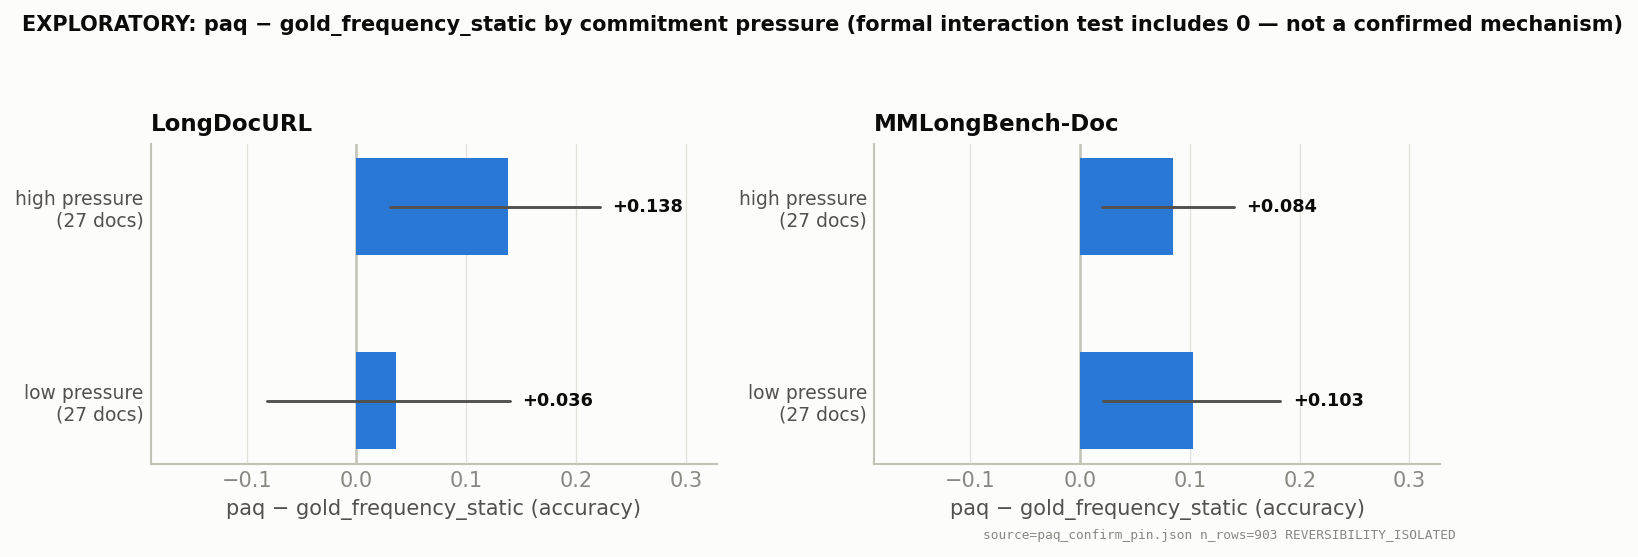
\includegraphics[width=\linewidth]{fig_c_pressure_mechanism_light.png}
\caption{EXPLORATORY (demoted): \paq{}$-$\texttt{gold\_frequency\_static} by commitment-pressure
split. The formal high$-$low interaction includes zero on both contrasts; shown for completeness,
not as a confirmed mechanism.}
\label{fig:pressure}
\end{figure}

% ----------------------------------------------------------------------------
\subsection{\paqt{}: training-free CV recall result --- accuracy pending}\label{sec:results-paqt}

\statusbox{PARTIAL / PENDING}{Expert-head + higher-resolution scoring descriptively meets or
exceeds the ColQwen2 RECALL means. This is neither a paired non-inferiority result nor accuracy:
the read-eval has not been run, and the expert-head technique is CAPS's.}

The \paqt{} gate (score-only; no reads) asks whether the recall deficit behind the $-$10pt loss is
an artifact of mean aggregation and scoring resolution. Its predeclared engineering verdict is
\texttt{PAQ\_T\_VIABLE}: the worst displayed per-cell gap to ColQwen2 is $-0.96$pt, inside the
10-point viability threshold. Held-out-document expert-head recall@$b{=}5\%$ is \textbf{0.674}
(LongDocURL, $n=451$) and \textbf{0.628} (MMLongBench-Doc, $n=425$). ColQwen2's in-harness means
are 0.664 and 0.536 (reference-pipeline values 0.694/0.555).

These are \emph{not} paired estimates on identical rows: \paqt{} covers 876 high-resolution-score
rows, whereas the coarse-\paq{} and ColQwen2 means use all 903 complete rows. Accordingly,
Table~\ref{tab:paqt} is a descriptive diagnostic, not a confidence-interval-backed parity test.
Within the displayed sequence, the largest change is from high-resolution mean aggregation
(0.523/0.460) to the cross-validated expert head (0.674/0.628); the coarse-to-high-resolution
increment cannot be cleanly attributed without recomputing both on the same 876 rows. Selected
heads lie in layers 18--21 (head $(21,10)$ is selected in one fold of each cell).

\begin{table}[t]
\centering
\small
\caption{\paqt{} page-selection recall@$b{=}5\%$ diagnostic. Sample sizes differ, so rows should
not be read as paired deltas. \textbf{This is recall, not answer accuracy}; the read-eval is
pending.}
\label{tab:paqt}
\begin{tabular}{lcc}
\toprule
Scorer & LongDocURL & MMLongBench-Doc \\
\midrule
coarse mean aggregation (\paq{} v1) & 0.494 ($n=463$) & 0.443 ($n=440$) \\
higher-resolution mean aggregation & 0.523 ($n=451$) & 0.460 ($n=425$) \\
expert head (held-out-document CV) & 0.674 ($n=451$) & 0.628 ($n=425$) \\
ColQwen2 in-harness reference & 0.664 ($n=463$) & 0.536 ($n=440$) \\
\bottomrule
\end{tabular}
\end{table}

Four caveats are load-bearing: (1) \textbf{recall parity $\neq$ accuracy parity} --- the
read-eval (reread expert-head top-$B$ pages, score against ColQwen2) is the required next
experiment, and until it runs \paqt{} has no accuracy claim; (2) \textbf{expert-head selection is
gold-supervised cross-validation and CAPS's method} \citep{zhu2026caps} --- no model weights are
trained, but gold recall on the complementary benchmark fold chooses the head, and our residual
novelty is the amortized one-prefill-many-queries architecture rather than the selector; (3) the
available-case mismatch above prevents an inferential non-inferiority claim; and (4) scoring
resolution was capped by encoder OOM (6{,}000-token target), so the resolution lever remains
under-tested. The result supports running the read-eval; it does not establish page-router parity.

% ----------------------------------------------------------------------------
\subsection{Efficiency framing (measurement pending)}\label{sec:results-efficiency}

\statusbox{UNMEASURED}{No latency/VRAM/throughput table exists yet. Everything in this subsection
is an accounting argument, flagged as such, with the red-team's caveats folded in.}

\paq{} is training-free, uses no separate retriever model and no multi-vector index; the coarse
prefill is paid once per document and each query costs one short forward over the retained cache
plus the reread. But the honest accounting (from the efficiency red-team) is: ColQwen2
\emph{also} amortizes (page embeddings are computed once; a query costs a small query encoding
plus MaxSim), and \paq's per-query readout is a reader-scale forward --- likely \emph{more}
per-query FLOPs than ColQwen2's query encoding. What \paq{} genuinely saves is
\emph{dependencies}: no second model resident, no index storage, one deployed artifact. Where the
amortization argument has real teeth is against CAPS, which re-forwards every page per query
(11.25\,s/query reported) and explicitly concedes the multi-query regime to embedding methods.
An efficiency-only justification while losing $\approx$10 accuracy points was reviewed as
weak-reject; we therefore make no efficiency claim until (a) the measured table exists
(cold/warm start, retriever co-resident vs.\ sequential, index bytes/page, several
queries-per-document), and (b) \paqt{} accuracy lands within the predeclared non-inferiority bars
(within 2--3 points, $\lb > -0.03$, both cells).

% ============================================================================
\section{Related work}\label{sec:related}

\subsection{CAPS: the page-level method is already published}\label{sec:related-caps}
\textbf{CAPS} \citep{zhu2026caps} (``Attention as Selector'', ACL~2026) publishes attention-based
page selection for long-document retrieval \emph{on our exact benchmarks}: a small scoring VLM's
final-token$\to$page attention at a single expert (layer, head), lightly calibrated on 6.4k
off-benchmark contrastive triplets, beats ColPali-pipeline retrieval (MMLongBench R@5 78.89 vs.\
72.00; downstream QA 44.69 vs.\ 36.18--41.01). Their training-free ablation lands just \emph{below}
ColPali (best zero-shot head R@5 70.92 vs.\ 72.00) --- independently corroborating our own
training-free loss. We state plainly: \textbf{the ``reader-attention selects pages'' method is
scooped}, and any contribution of ours must be argued elsewhere. CAPS's own concessions define
the open ground: it scores every page independently per query (multi-query latency conceded to
embedding methods --- exactly \paq's amortized regime) and operates at page granularity only
(region-level selection named as an open problem --- exactly extension E1).

\subsection{KV compression and eviction}
H2O \citep{zhang2023h2o}, SnapKV \citep{li2024snapkv}, FastV \citep{chen2024fastv}, LOOK-M
\citep{wan2024lookm}, and KVzip \citep{kim2025kvzip} commit a compressed cache once; Quest
\citep{tang2024quest} shows query-aware beats query-agnostic at tight budgets in single-query
text --- motivation for, but not evidence of, our multi-query claims. SparseVILA
\citep{sparsevila2025} is the nearest VLM neighbor for extension E2 (prefill pruning + decode-time
retrieval) but prunes irreversibly at prefill and never compares against retrieval pipelines on
long-document VQA; Kamera \citep{kamera2026} shows the multi-query KV-reuse serving regime is
becoming real.

\subsection{Trained visual retrieval}
ColPali/ColQwen2 \citep{faysse2025colpali} is the strong deployable retriever we lose to; M3DocRAG
\citep{cho2024m3docrag} and successors are the pipelines CAPS beat. The bar is moving:
ColQwen3-class models and small distilled retrievers keep improving, so even a future win over
ColQwen2 must be argued as a mechanism/regime result, not a leaderboard entry. A published
oracle-analysis on MMLongBench \citep{hybridretriever2026} mirrors our fusion finding
(best-per-query routing between retrievers gains $+0.9$; union reranking gains more), and
attention-based reranking precedents exist in text \citep{chen2025icr,wu2025qrhead}.

\subsection{Benchmarks and the region-level neighborhood}
MMLongBench-Doc \citep{ma2024mmlongbench} and LongDocURL \citep{deng2025longdocurl} supply the
multi-query long-document structure; MMDocIR \citep{mmdocir2025} adds layout-level retrieval
labels useful for E1's localization sanity checks. The region-level neighborhood is active ---
RegionRAG \citep{regionrag2025} (trained retriever-side crops; near-flat on long docs, no long-doc
QA), Snappy \citep{snappy2025} (training-free patch$\to$OCR-box propagation, localization only),
AGREE \citep{agree2025} (reader attention distilled into a trained retriever), VRAG-RL
\citep{vragrl2025} and Doc-V* \citep{docvstar2026} (agentic crop/zoom loops), ViCrop/FOCUS
\citep{vicrop2025,focus2025} (single-image training-free cropping). In our current search we did
\textbf{not identify prior work in the exact combined cell}: reader-internal attention as the
runtime region selector, end-to-end QA at matched token budget vs.\ page-level retrieval, on long
documents, multi-query amortized. This is a provisional literature-map claim, not proof of
novelty; it motivates the E1 proposal. Page-selection-then-read itself long predates us
\citep{mpdocvqa2024}.

% ============================================================================
\section{Current state, open questions, roadmap}\label{sec:roadmap}

\subsection{Scoreboard (2026-07-15)}
\begin{center}\small
\begin{tabular}{lll}
\toprule
Item & Status & Where \\
\midrule
Multi-query reversibility isolation (page level) & \textbf{CONFIRMED} (903 q, both cells) & \S\ref{sec:results-isolation} \\
Executed retrieval-vs-selection panel at 64K & \textbf{DONE} (first of its kind, to our knowledge) & \S\ref{sec:baselines}, App.~\ref{app:panel} \\
\paq{} vs.\ ColQwen2-fresh & \textbf{LOST} ($-0.099$ pooled) & \S\ref{sec:results-retrieval} \\
Page-level attention selection as a method & \textbf{SCOOPED} (CAPS, ACL 2026) & \S\ref{sec:related-caps} \\
Commitment-pressure mechanism & \textbf{DEMOTED} (interaction test incl.\ 0) & \S\ref{sec:results-mechanism} \\
\paqt{} zero-shot recall parity & \textbf{CONFIRMED (recall only)} & \S\ref{sec:results-paqt} \\
\paqt{} accuracy read-eval & \textbf{PENDING} (the next experiment) & \S\ref{sec:results-paqt} \\
Efficiency table & \textbf{PENDING} (unmeasured) & \S\ref{sec:results-efficiency} \\
E2 PAQ-KV (token-level reversible KV) & \textbf{ROADMAP}, odds $\sim$25--35\% & \S\ref{sec:method-extensions} \\
E1 PAQ-Fovea (region-level foveation) & \textbf{ROADMAP}, odds $\sim$15--25\% & \S\ref{sec:method-extensions} \\
\bottomrule
\end{tabular}
\end{center}

\subsection{The thesis going forward}
\begin{figure}[t]
\centering
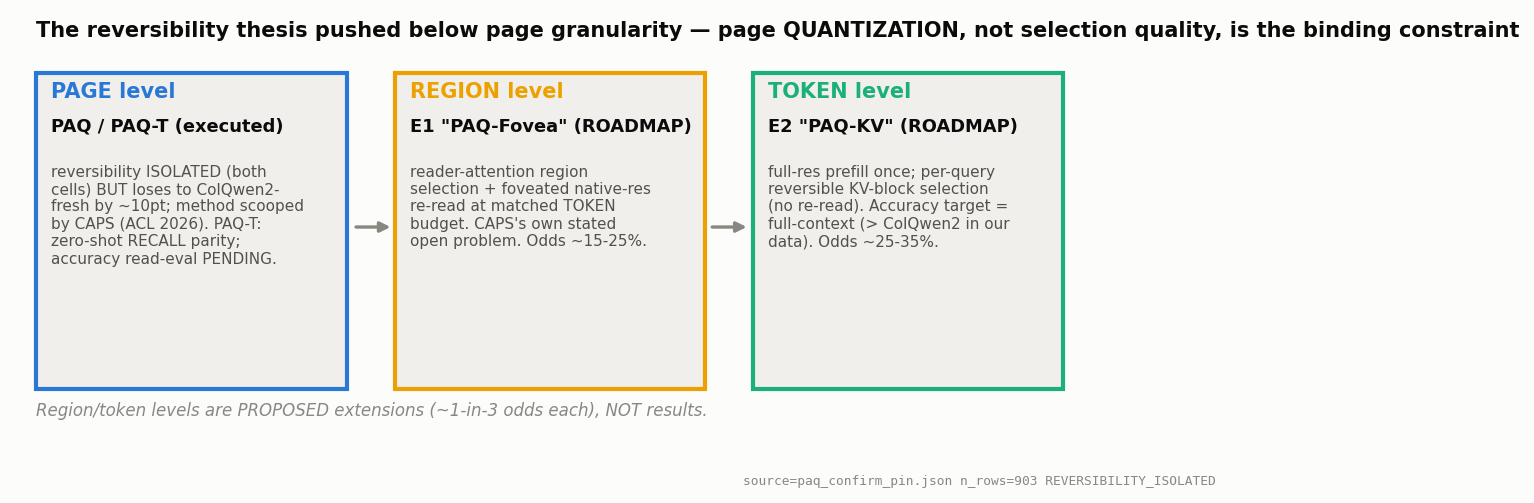
\includegraphics[width=\linewidth]{fig_g_granularity_schematic_light.png}
\caption{The page $\to$ region $\to$ token reversibility roadmap. Page level is executed (and
lost/scooped); region and token levels are \emph{proposals} at $\sim$1-in-3 odds each. The
unifying observation: retrieval quantizes evidence to whole pages, so at a fixed budget the open
opportunity is below page granularity, where a reader that has already prefilled the document can
re-select reversibly per query.}
\label{fig:schematic}
\end{figure}

The reframe that survived every review round: \textbf{page quantization, not selection quality,
is the binding constraint}. ColQwen2 wins the page-ranking game, and CAPS owns the attention
variant of it --- but a whole-page budget is wasteful (most of a kept page is not evidence), and a
page-level index cannot re-allocate budget within pages. The reader's retained prefill can. The
two proposed operating points (Figure~\ref{fig:schematic}):
\begin{itemize}
  \item \textbf{E2 / PAQ-KV (token):} the best-priced bet --- its accuracy target (full-context)
        already beats ColQwen2-fresh in our own data ($+0.033$/$+0.069$), so it needs selection
        loss $<\sim$1pt rather than a swing. Risks: a 2--4 day engineering spike (Qwen3-VL
        block-top-k under M-RoPE/DeepStack), and the LongDocURL margin ($+0.033$) is inside our CI
        half-width --- a per-cell $\lb>0$ there requires landing essentially at full-context.
  \item \textbf{E1 / PAQ-Fovea (region):} the highest-novelty bet (CAPS's own named open problem;
        the cell is unoccupied, \S\ref{sec:related}); needs the largest accuracy swing
        ($\sim$$+0.14$ total) and its localization sanity at coarse resolution is unproven.
\end{itemize}
Both are \textbf{$\sim$1-in-3 propositions and are stated as such}. If neither survives its
cheap screen, the honest terminus of this program is what is already in this document: the
reversibility regime result, the executed panel, and the boundary map.

\subsection{Open questions}
(1) Does \paqt{} recall parity convert to accuracy non-inferiority (the pending read-eval)?
(2) Does the E2 spike land, and does token-level selection preserve full-context accuracy on
multi-hop/cross-page questions (Quest-family methods degrade exactly there, and MMLongBench-Doc
is 33\% cross-page)? (3) Can coarse-prefill heatmaps localize regions at all (E1's gate)?
(4) The moving bar: ColQwen3-class retrievers may outdate any ColQwen2 comparison by submission
time --- any win must be a regime/mechanism claim. (5) A second VLM (currently everything is a
Qwen3-VL-8B case study).

% ============================================================================
\section{Limitations}\label{sec:limitations}
\begin{itemize}
  \item \textbf{Heterogeneity.} Effect sizes differ by cell (e.g.\ the stale gap is $+0.257$ vs.\
        $+0.163$); we never average cells except in the labelled pooled statistic, and per-cell
        results are primary.
  \item \textbf{Page routing only.} v1 selects pages and rereads at full resolution; it is not KV
        compression, makes no memory/latency claim, and the systems-level story is unmeasured
        (\S\ref{sec:results-efficiency}).
  \item \textbf{Base-model ceiling.} 35.1\% of confirmatory queries are oracle-unanswerable
        (score 0 given exactly the gold pages); only 45.1\% are fully oracle-answerable. Absolute
        numbers are deflated for every arm; oracle is not a strict ceiling (28 \paq{} wins over it).
  \item \textbf{Resolution cap.} The high-res vision encoder OOMs on many-page documents, so
        \paqt{} scoring was capped at a 6{,}000-token target --- the resolution lever is
        under-tested and a \paqt{}-negative would have been inconclusive.
  \item \textbf{CAPS overlap.} Expert-head attention selection is CAPS's published method; any
        \paqt{} claim is limited to the amortized multi-query architecture and must credit CAPS.
  \item \textbf{Recall $\neq$ accuracy.} The only \paqt{} evidence is recall; the accuracy
        read-eval is pending and could fail.
  \item \textbf{Weak family ports.} FastV/LOOK-M/KVzip are disclosed proxies and SnapKV is a weak
        port; we claim nothing against canonical versions of them.
  \item \textbf{Single reader.} All results are a Qwen3-VL-8B case study; generalization to other
        VLMs is untested.
  \item \textbf{Stale-policy dependence.} The commit-once aggregate uses the first
        $M{=}\min(3,k)$ queries in frozen arrival order; order-permutation and $M$-sensitivity
        robustness checks were reviewer-requested and remain to be run (the gold-informed static,
        which is order-free, partially covers this).
\end{itemize}

% ============================================================================
\appendix
\section{Full executed panel at the gate budget}\label{app:panel}

\begin{table}[h]
\centering\small
\caption{Every arm, accuracy at $b{=}5\%$, per cell (verbatim from
\texttt{research/paq\_verdict.json}). The query-blind family sits at/below random gold-recall ---
the anti-strawman record: beating it is visibly not the claim.}
\label{tab:panel}
\begin{tabular}{llcc}
\toprule
Group & Arm & LongDocURL & MMLongBench-Doc \\
\midrule
\multirow{2}{*}{ours}
 & \paq{} & \textbf{0.386} & \textbf{0.258} \\
 & attn\_max (alt-agg) & 0.337 & 0.152 \\
\midrule
\multirow{2}{*}{isolation}
 & paq\_stale (commit-once) & 0.128 & 0.095 \\
 & gold\_frequency\_static & 0.278 & 0.154 \\
\midrule
\multirow{3}{*}{deployable retrieval}
 & ColQwen2-fresh & 0.512 & 0.328 \\
 & ColQwen2-stale & 0.216 & 0.138 \\
 & CLIP-fresh & 0.155 & 0.164 \\
\midrule
\multirow{3}{*}{reference (not competitors)}
 & SnapKV-fresh & 0.298 & 0.157 \\
 & full-context & 0.546 & 0.397 \\
 & oracle-evidence (not strict) & 0.609 & 0.431 \\
\midrule
\multirow{7}{*}{query-blind controls}
 & SnapKV-stale & 0.083 & 0.074 \\
 & H2O & 0.045 & 0.039 \\
 & FastV (ctx-only proxy) & 0.045 & 0.031 \\
 & LOOK-M ($\to$H2O on images) & 0.045 & 0.039 \\
 & KVzip (recv\_max proxy) & 0.047 & 0.048 \\
 & random & 0.068 & 0.022 \\
 & truncation & 0.033 & 0.041 \\
\bottomrule
\end{tabular}
\end{table}

Secondary statistics (pooled, reported not gated): \paq{} beats the best family arm
(SnapKV-stale) with min-over-family $\lb = +0.202$; \paq{} $-$ SnapKV-fresh $= +0.094$
$[+0.069, +0.122]$; \paq{} $-$ attn\_max $= +0.077$ $[+0.048, +0.110]$; \paq{} $-$ oracle
$= -0.199$ $[-0.239, -0.161]$.

Gold-page recall at $b{=}5\%$ (per cell, LongDocURL / MMLongBench-Doc): \paq{} 0.494/0.443;
\texttt{gold\_frequency\_static} 0.381/0.373; \texttt{paq\_stale} 0.137/0.148; ColQwen2-fresh
0.664/0.536.

\section{The adversarial review trail (anti-strawman record)}\label{app:reviews}
This project's positives were only believed after surviving independent cross-family review; two
of them did not survive, and we list the retractions because they are part of the evidence:
\begin{enumerate}
  \item \textbf{Pre-freeze design review} (code-faithfulness + methodology, 2026-07-14): folded
        best-of-family gating, document-cluster bootstrap, the page-routing estimand disclosure,
        first-$M$ stale aggregation, and power floors \emph{before} any GPU run.
  \item \textbf{v1 gate retraction.} The first gate (\texttt{PAQ\_V1\_GO}, \paq{} beats
        the eviction family) \emph{passed and was then retracted}: reviewers + an independent
        reproduction showed a gold-informed static nearly matched \paq's recall --- the family's
        weakness was a weak-static artifact, and reversibility had not been isolated. The
        two-comparator isolation gate (Eq.~\eqref{eq:gate}) replaced it and was frozen before
        the re-run.
  \item \textbf{Result review of the isolation positive} (2026-07-14): heterogeneity honestly
        surfaced (screen-scale MMLongBench static contrast $-0.017$, CI incl.\ 0 --- later
        resolved at 80 docs); \texttt{attn\_best}, a derived arm that peeked at gold task
        score, was dropped.
  \item \textbf{Final AAAI-readiness review} (2026-07-15): named the missing deployable retrieval
        baseline as the \#1 threat --- running it produced the decisive loss
        (\S\ref{sec:results-retrieval}); forced the \texttt{best\_static} $\to$
        \texttt{gold\_frequency\_static} rename and the $\lb$ relabel; demoted the mechanism
        claim (\S\ref{sec:results-mechanism}); required the independent-extension and
        missingness analyses (\S\ref{sec:results-isolation}).
  \item \textbf{Efficiency red-team} (2026-07-15): rejected efficiency-only framing
        (\S\ref{sec:results-efficiency}) and predeclared the non-inferiority bars \paqt{} must
        meet.
\end{enumerate}

\section{Reproducibility}\label{app:repro}
\begin{itemize}\small
  \item \textbf{Harness} (frozen): \texttt{scripts/paq.py} (v1 sha256 \texttt{735eecaa\ldots},
        commit \texttt{ca66292}; v2 \texttt{e9e06aad\ldots}, commit \texttt{f7e7a53}; v3 = v2 +
        confirmatory pin, re-scored at commit \texttt{b653e85}). Retrieval arms:
        \texttt{scripts/paq\_retrieval\_arms.py} (ColQwen2 \texttt{vidore/colqwen2-v1.0} + CLIP;
        incremental merge --- the frozen gate math and the retrieval-free rows are untouched).
        \paqt{} gate: \texttt{scripts/paq\_t\_gate.py}. Figures: \texttt{scripts/paq\_figs.py}
        (all numbers read from the verdict JSONs; every figure carries a source stamp
        \texttt{pin\,$\cdot$\,n\_rows\,$\cdot$\,verdict}).
  \item \textbf{Pins}: screen \texttt{research/paq\_pinned\_subset.json} (sha256
        \texttt{b194ed84\ldots}, chmod 444, byte-verified by the harness); confirmatory
        \texttt{research/paq\_confirm\_pin.json} (80 docs/cell; the screen pin is its prefix).
  \item \textbf{Verdicts}: \texttt{research/paq\_verdict.json} (gate + budget curves + retrieval
        secondary + strata), \texttt{research/paq\_t\_gate\_verdict.json}; per-query per-arm rows
        in \texttt{research/paq\_results.jsonl}; cached retrieval scores in
        \texttt{research/paq\_retrieval\_scores.json}.
  \item \textbf{Gate + bootstrap + pairing} are unit-tested (\texttt{paq.py --selftest}); the
        belief gate, arm classifications, and strata were pre-registered in the frozen bar.
  \item \textbf{Commands}: gate \texttt{python scripts/paq.py --run --cell vision --gate-only};
        full contest \texttt{--run --cell all}; scoring \texttt{--score}; figures
        \texttt{python scripts/paq\_figs.py}.
\end{itemize}

\section{Timeout recovery note}\label{app:timeout}
The confirmatory hit its 10-hour wall-clock limit during final scoring (exit 124) at 903/907
vision queries. Because the harness flushes each row as it completes, the run was recovered by
re-scoring the flushed rows on CPU (no GPU re-run, no selection re-computation); the 4 unscored
queries are the \texttt{mi\_phone} rows of \S\ref{sec:results-missing}, and the worst-case
imputation leaves every gate conclusion unchanged. A separate single-query text cell
(``counting'') was truncated by the same timeout and is out of scope for the multi-query claims;
it was not re-run.

\bibliographystyle{aaai2027}
\bibliography{references}

\end{document}
